% Research Map article: sections 1-7 drafted (C163).
% Target journal: Information Processing & Management. No journal template assumed.
\documentclass[11pt,a4paper]{article}
\usepackage[T1]{fontenc}
\usepackage[utf8]{inputenc}
\usepackage[english]{babel}
\usepackage{geometry}
\usepackage{array}
\usepackage{graphicx}
\usepackage{url}
\geometry{margin=28mm}

\newcommand{\outlinenote}[1]{\par\smallskip\noindent\textit{Planned content: #1}\par\medskip}

\title{The Research Map: A Method and Human-Supervised AI System for Structuring Research Plans}
\author{S{\'e}rgio Luiz Braga Fran\c{c}a$^{a}$ \quad Mario Reis$^{b}$\\[0.6em]
\small $^{a}$Escola de Engenharia, Universidade Federal Fluminense (UFF)\\
\small Campus da Praia Vermelha, Rua Passo da P\'atria, 156, S\~ao Domingos\\
\small Niter\'oi, RJ 24210-240, Brazil\\[0.25em]
\small $^{b}$Instituto de F\'isica, Universidade Federal Fluminense (UFF)\\
\small Av. Gal. Milton Tavares de Souza, s/n\textsuperscript{o}, Campus da Praia Vermelha\\
\small Niter\'oi, RJ 24210-346, Brazil}
\date{Working draft, 30 October 2026}

\begin{document}
\maketitle
\begin{abstract}
Research plans require explicit relationships among a central problem, objectives, literature, planned methods, and expected outputs. This article describes the Research Map, a five-stage method with a companion objective--method matrix, and examines its operationalization in a human-supervised AI application. We analyze two primary methodological documents, inspect the relevant software implementation and local technical checks, compare related scholarly systems and publicly documented applications, and present a constructed illustrative walkthrough. The application represents planning units as editable proposals and confirmed content, records links and revisions, marks dependent element types for reconsideration, and supports conditional advisor review of student submissions. The walkthrough shows how a hypothetical change to a research problem would call for renewed inspection of objectives, topics, and methods; it is not an observed application session. The contribution is a traceable account of the correspondence between this particular method and its implemented workflow, including incomplete translations: research questions have no dedicated unit, revision impact is determined by element type rather than exact links, and the final coherence review is advisory. These descriptions do not establish scientific validity, usability, improved planning quality, or time savings. The resulting map is a revisable planning artifact whose methodological adequacy remains a human judgment.
\end{abstract}
\noindent\textbf{Keywords:} research planning; research methodology; human-AI collaboration; AI-assisted authoring; traceability.

\section{Introduction}
\label{sec:introduction}

A research plan contains more than a topic and a collection of well-formed sentences. Its central problem, objectives, literature topics, planned methods, and expected outputs need intelligible relationships if the plan is to be examined and revised. A practical difficulty motivating the Research Map is that these components can be drafted separately without making their connections clear. Sergio Fran\c{c}a's teaching map and later methodological specification address that difficulty by relating five planning stages to a companion objective--method matrix and by calling for human validation of proposed content \cite{franca2026map,franca2026detail}. This motivation identifies a design problem; it does not establish how often researchers encounter it or whether a structured map reduces delays or improves their work.

AI-supported research tools already address adjacent tasks. Published systems assist with staged proposal development, formulation of research questions, generation and critique of research ideas, and inspection of revision histories \cite{guerard2026researchllm,wang2026fivestage,liu2024coquest,baek2025researchagent,freire2006vistrails}. Publicly documented planning applications also describe persistent records, review checkpoints, or revision assistance \cite{projectready2026guide,researchly2026site}. These antecedents make generic claims about an agent, a sequence of prompts, or human oversight insufficient to distinguish the present work. The question for this article is more specific: \emph{How are the Research Map's methodological relationships represented and supported in a human-supervised AI application, and where does that representation remain incomplete?}

We address the question as a method-and-system account. First, we describe the Research Map from its two author-supplied methodological documents, separating the five numbered stages from the accompanying matrix and from later proposals for software support. Second, we examine the inspected implementation: editable AI proposals, confirmed planning units, links, revisions, checks, conditional advisor review, and export. The unit of analysis is the correspondence between methodological relations and software structures, including mismatches between them. Our contribution is a documented, inspectable account of the correspondence between a particular planning method and its current application, together with the limits of that correspondence. We do not claim that its individual functions are unprecedented or that the software validates a research design scientifically.

The evidence combines the primary method documents, a focused narrative comparison with scholarly work and publicly described applications, inspection of relevant source code and local technical checks, and one constructed walkthrough. The walkthrough uses a fictional library project to show how an upstream change could prompt reconsideration of objectives, topics, and the matrix. It is an explanatory example, not an application session or a study with participants. No user outcomes, methodological ratings by the authors, time savings, or comparative effectiveness are reported. This scope permits a critical account of what the method specifies and what the inspected system supports, while leaving questions of use and impact for separate empirical work.

Section~\ref{sec:state-of-the-art} positions the work among research-planning agents, provenance systems, and public applications. Section~\ref{sec:method} presents the Research Map method; Section~\ref{sec:system} examines its operationalization in the application and agent. Section~\ref{sec:walkthrough} gives the constructed example, followed by the contribution boundary and limitations in Section~\ref{sec:discussion} and the conclusion in Section~\ref{sec:conclusion}.

\section{State of the art}
\label{sec:state-of-the-art}

The literature relevant to the Research Map spans different units of work: formulating a question, generating a research idea, organizing a full project, and preserving the history of revisions. Similar interface features do not imply equivalent methodological purposes. This is a focused narrative review of seven supplied scholarly papers and the PROV-DM standard, complemented by public documentation for six applications; it is not a systematic search or a functional evaluation of those applications. We compare the artifact produced, the human researcher's role, the treatment of revisions, and the connection to the Research Map.

\subsection{From an initial problem to a research design}

Guerard et al. propose Research LLM as a three-stage human-in-the-loop framework covering proposal development, research design, and manuscript preparation \cite{guerard2026researchllm}. Their account combines prompting and verification techniques with explicit human checkpoints; it illustrates the pipeline through a hiring-bias case and reports an exploratory, qualitative pilot with master's students developing thesis proposals. The paper is close to the Research Map in treating the researcher as the decision maker across several stages. Its organizing artifact, however, is a broad research pipeline rather than a specified map linking a central problem, a general objective, specific objectives, chapter topics, and a collection--analysis--expected-result entry for each objective. The distinction concerns the structure being documented, not the presence of human review.

Wang et al. offer a more directly methodological comparator \cite{wang2026fivestage}. Their five-stage approach begins with observation and appraisal of a problem in general practice, transforms it into searchable concepts, summarizes the literature, constructs a research-question prototype, and then considers methodology and feasibility. Tables and prompts carry information between stages; clinicians inspect and amend intermediate outputs. The authors report feedback from a panel of ten general-practice researchers and one worked process log, rather than a controlled effectiveness trial. Both approaches connect a practical problem to literature and method, but their five stages are not the same five stages. Wang et al. organize the path toward a clinical research question; the Research Map organizes a project through problem, general and specific objectives, literature and development topics, with an accompanying objective--method matrix. The latter matrix asks separately what will be collected, how it will be analyzed, and what result is expected for each objective. An expected result is a planning entry, not an empirical finding.

CoQuest narrows the unit of assistance to research-question ideation \cite{liu2024coquest}. Its interface displays a flow of candidate questions, related literature, and the agent's rationale; users can explore breadth-first or depth-first alternatives and provide feedback. A within-subjects study with 20 HCI researchers compared those interaction designs and reported differences in perceived creativity and trust. CoQuest thus provides evidence about human--AI interaction during question generation that the present article cannot claim for the Research Map. Conversely, its evaluated task is not the maintenance of a project-wide objective--method plan. Research questions are relevant to the detailed Research Map method, but they are not a sixth numbered stage of its original five-stage structure; the current application also lacks a separate research-questions unit. This difference prevents us from treating CoQuest's user findings as evidence for our system.

\subsection{Agentic generation and critique}

ResearchAgent starts from a scientific paper and related literature, then proposes a problem, method, and experimental design; reviewing agents critique successive versions \cite{baek2025researchagent}. The authors compare model variants using human and model-based judgments of generated ideas. This work already joins literature grounding, methodological proposals, and iterative agent critique. Its primary artifact is an automatically generated research idea, whereas the Research Map is a researcher-maintained arrangement of linked project components. The comparison also exposes a shared risk: a plausible proposed method still requires substantive checking by a domain expert. ResearchAgent's evaluation results cannot be transferred to the Research Map, whose proposals, checkpoints, and outcomes have not been tested in that study.

Intelliscope, described by Aamer et al., connects biomedical entities through knowledge-graph paths and uses Analyst, Scientist, and Reviewer agents to explain those paths, design predictors and validation experiments, and refine proposals \cite{aamer2026biomedical}. Its ResearchMemory records design iterations and reviewer feedback, and its dashboard supports inspection of the generated work. It is a stronger comparator for retained agent decisions than a generic chatbot. Its knowledge-graph inputs and biomedical discovery outputs differ substantially from the Research Map's general project-planning fields. Consequently, neither multiple agent roles, retained feedback, nor human oversight can serve as the article's standalone novelty claim; the issue is how a particular methodological plan is represented and revised in the implemented workflow.

\subsection{Provenance and revision of structured artifacts}

VisTrails records actions that transform one scientific workflow into another and arranges workflow versions in a tree, allowing prior configurations and outputs to be revisited \cite{freire2006vistrails}. The W3C PROV-DM recommendation supplies a domain-independent account of entities, activities, agents, and derivations \cite{moreau2013prov}. RaivenTracks applies a more recent version-history design to conversational visualization: validated visualization specifications become branchable checkpoints, with a separate undo/redo layer for runtime settings \cite{hugie2026raiventracks}. RaivenTracks is a preprint; its formative pilot involved three visualization researchers and had no comparison baseline.

These sources clarify what the Research Map can mean by traceability. A record of a proposed field, its source revision, the researcher's decision, and the later version makes a change inspectable. It does not prove that the relation between a problem and an objective is scientifically sound. Unlike the workflow or visualization artifacts in VisTrails and RaivenTracks, the Research Map's objects are methodological statements and planning relations. In the current application, confirmed changes can mark downstream \emph{types} of component for review while preserving their text and history; this is conservative type-level invalidation, not an exact causal graph of every affected statement. PROV-DM is a conceptual comparator, not a claim that the application implements the W3C model in full.

\subsection{Applications documented outside the research literature}

The academic texts are not the whole landscape of practice. In this focused scan, ProjectReady AI is the closest publicly documented product comparator: its guide describes a persistent Research Record with approved objectives, questions, design decisions, researcher checkpoints, supervisor corrections, and an alignment audit \cite{projectready2026guide}. Researchly AI likewise advertises a path from research idea to plan, literature and method support, trust labels, supervisor review, and a ``what-if'' operation that recalculates parts of a plan after a change \cite{researchly2026site}. These are substantial overlaps with the Research Map's authoring and revision goals. Their public pages do not disclose enough internal behavior to determine whether their dependency rules are equivalent to the Research Map's, and we did not test authenticated workflows. It would therefore be unsound to claim either that these products lack such rules or that the Research Map is the first persistent AI-assisted research planner.

Other tools illustrate narrower or adjacent overlaps. Bodhi's Proposal Builder advertises generation of gaps, problem statements, objectives, hypotheses, methods, and expected outcomes from a topic \cite{bodhi2026proposal}. ResearchPlanBuilder's public repository describes guided planning questions, an optional AI step, a browser-local draft, and a generated research plan \cite{vallavaraj2026builder}. Reos plans user and product research through objectives, methods, participant criteria, questions, and a moderation guide, and its product page says that later evidence is linked back to those questions \cite{reos2026plan}. Tykyra structures a systematic literature review from protocol and search terms through screening and export, with claimed auditability of review decisions \cite{tykyra2026site}. The first two overlap with proposal construction; Reos overlaps with question-to-evidence links in another research domain; Tykyra concerns execution of a literature-review protocol rather than organization of a whole research project. These statements describe vendor documentation or a repository README, not independently verified operation, comparative performance, or proof that any product has no associated scholarly publication.

\subsection{Connection to the Research Map and contribution boundary}

Taken together, the comparisons locate the Research Map between question ideation, agent-supported design, and revision of structured artifacts. The method supplies a specific sequence: one central problem, an aligned general objective, specific objectives, literature and development topics, and a companion matrix connecting each objective to planned collection, analysis, and expected result. The article's system contribution is to describe how these relations become editable proposals, human confirmation points, stored links, versioned revisions, and review cues in the application. The illustrative walkthrough will show one constructed change moving through that arrangement; it will not stand in for a user study or an observed research outcome.

This boundary matters for the comparison. The cited papers and products already cover staged prompting, question exploration, agent critique, memory, review checkpoints, exports, and provenance in various combinations. The defensible contribution is an inspectable account of the translation of this particular method into its current application and agent, including where the translation is incomplete. In particular, the application's lack of a dedicated research-question unit, type-level rather than exact dependency invalidation, and advisory final coherence review constrain what can be claimed about methodological fidelity. Neither the reviewed literature nor the present descriptive case establishes superiority, general effectiveness, or automatic scientific validity.

\section{The Research Map method}
\label{sec:method}

\subsection{Origin, sources, and purpose}

The Research Map is a method for structuring a proposed academic research project. Its primary source is a teaching map prepared by Sergio Fran\c{c}a in August 2026; a subsequent methodological specification makes the intended dependencies and review points more explicit \cite{franca2026map,franca2026detail}. The method is motivated by a practical planning difficulty: a broad theme, a central problem, objectives, chapter topics, and methods can be drafted separately without a clear account of how one leads to another. A later author-supplied application export articulates this concern in terms of students' difficulty beginning and organizing a project. We treat that account as a design motivation, not as a measured frequency of difficulties, delays, or educational outcomes.

The two primary documents have different roles. The initial map is a compact template that numbers five stages and places the objective--method matrix beside the specific objectives. The later specification describes rules of dependency, an origin--destination traceability map, coherence questions, and points at which a researcher may validate or revise proposed content. Some passages of the later document describe capabilities a supporting system \emph{should} have. In this section they are reported as part of the methodological specification, not as evidence that the application implements every capability. Section~\ref{sec:system} will examine that correspondence separately.

\subsection{Five stages and their relations}

The map begins with one central research problem: a question that gives the project its focus. The detailed specification suggests producing alternatives from the researcher's context, theme, or keywords, then selecting a definitive formulation for subsequent steps \cite{franca2026detail}. It recommends beginning that question with expressions equivalent to ``How'' or ``In what way''. This is a local drafting convention intended to elicit a researchable relation, not a universal requirement for scientific questions. The researcher's selection and revision of the problem remain substantive decisions.

A single general objective should respond to the selected problem and state the intended overall result of the project. The specification recommends an infinitive verb and uses the general objective as a basis for a provisional title \cite{franca2026map,franca2026detail}. The general objective is then decomposed into three to six specific objectives. Each should contribute a step toward the overall aim, rather than introduce an unrelated project. The detailed specification illustrates four specific objectives, but four is a suggested starting configuration within the original range, not a new fixed count.

The fourth stage organizes literature-review topics from the problem, keywords, and objectives. The initial map suggests three to six such topics. The fifth stage organizes development or analysis topics from the objectives, including the general objective where appropriate \cite{franca2026map}. A specific objective may be addressed principally through the literature review or through later development or analysis, depending on its role. The suggestion that a final development topic reconnect to the general objective is guidance for a coherent exposition, not a rule that every disciplinary article must follow. The map's stages describe relationships among planning elements; they need not be read as an irreversible sequence of writing operations.

\begin{table}[htbp]
\centering
\small
\caption{The five numbered stages in the original Research Map and their planning relations. The objective--method matrix is a companion element, not a sixth stage.}
\label{tab:method-stages}
\begin{tabular}{p{0.25\linewidth} p{0.34\linewidth} p{0.31\linewidth}}
\hline
Stage & Planning artifact & Principal relation \\
\hline
1. Research problem & One selected central question & Establishes the project's focus \\
2. General objective & One overall intended aim & Responds to the problem; informs the provisional title \\
3. Specific objectives & Three to six contributing steps & Decompose the general objective \\
4. Literature topics & Thematic review outline & Draws on the problem, keywords, and relevant objectives \\
5. Development / analysis topics & Outline for later analysis or development & Organizes the objectives to be addressed beyond the review \\
\hline
\end{tabular}
\end{table}

The detailed specification also treats research questions as an item for validation and revision \cite{franca2026detail}. They belong to the method's account of a research design, but they are not a sixth numbered stage in the initial map. This distinction matters when comparing the source method with the application, which presently has a central problem question but no separate research-questions unit.

\subsection{The objective--method matrix}

Beside the specific objectives, the original map places three planning questions: how information or data will be collected for each objective; how they will be analyzed or treated; and what result or impact is expected \cite{franca2026map}. This matrix connects a stated aim to a proposed means of addressing it. It can expose a missing collection procedure, an analysis that does not answer the objective, or an expected result that has no evident route from the planned work. These are issues for examination, not defects proven by the presence or absence of a filled cell.

The matrix is associated with the five stages rather than numbered as an additional stage. Its entries are prospective: \emph{expected result} names an anticipated output of a proposed study, not a finding already observed. In particular, completing this matrix does not establish that a method is feasible, that evidence will be obtained, or that an expected impact will occur. The researcher must judge the appropriateness of each collection and analysis choice in the project's disciplinary context.

\subsection{Dependencies, traceability, and human judgment}

The later specification represents the map as a set of origin--destination relations: inputs inform the selected problem; the problem informs the general objective; that objective informs the specific objectives; and the objectives guide literature and development topics \cite{franca2026detail}. It also proposes checking whether an objective has a corresponding topic, a plausible method, a collection procedure, an analysis, and an expected result. A traceability relation identifies why an item is present and what it is intended to address. It does not, by itself, establish conceptual coherence or scientific adequacy.

The specification therefore pairs suggested checks with researcher validation. The researcher may choose a problem from alternatives, adjust the general and specific objectives, revise research questions and topic structures, and assess the proposed methodological connections. The logic of dependency, traceability, coherence inspection, and human revision belongs to the method. A growing knowledge base, a comprehensive methodological library, and a rule engine are proposed means of supporting that logic; they are not additional numbered stages and should not be assumed to exist fully in the current software \cite{franca2026detail}.

\begin{figure}[htbp]
\centering
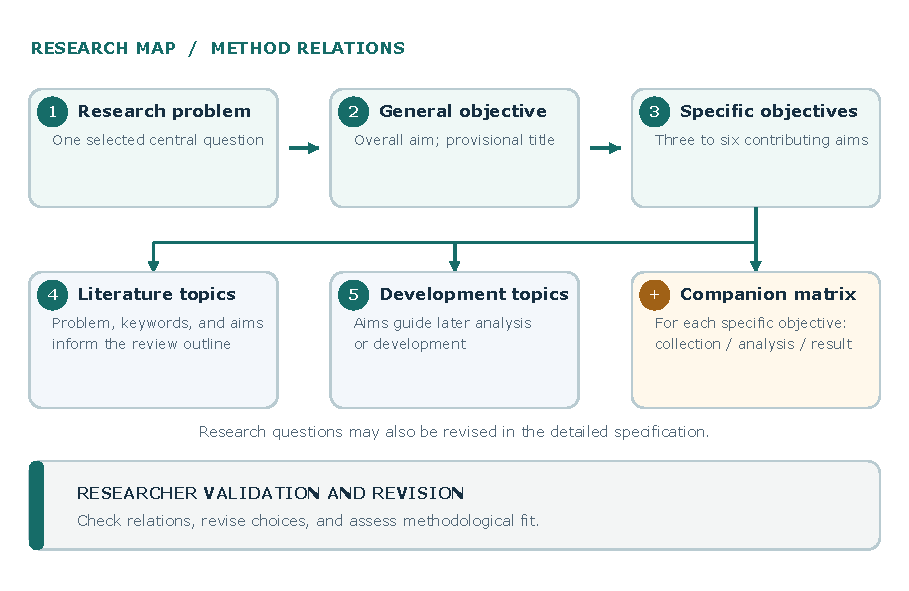
\includegraphics[width=\linewidth]{figures/method-flow.pdf}
\caption{Interpretive redrawing of the Research Map's five stages, companion matrix, and human revision. Arrows express methodological relations described in the primary documents; they do not represent observed application behavior or an irreversible workflow.}
\label{fig:method-flow}
\end{figure}

The method supplies a structured way to make planning decisions and their intended relations explicit. It does not offer a formal proof that a completed map yields a valid research design, nor does it evaluate the efficiency of planning. The next section examines which of these methodological relations are represented in the present application and agent, and where that representation is partial.

\section{Operationalization in the application and AI agent}
\label{sec:system}

\subsection{Scope and method-to-implementation correspondence}

This section describes the inspected version-2 implementation of the Research Map, rather than an observed pattern of use. The application turns the method's planning relations into an editable, versioned workflow. Its AI agent proposes text and comments on coherence; it does not decide whether a research design is scientifically adequate. Table~\ref{tab:method-system} separates method components present in the inspected code from partial translations and prospective capabilities. The terms in the table describe implementation, not an assessment of the method's effectiveness.

\begin{table}[htbp]
\centering
\small
\caption{Selected correspondences between the Research Map and the inspected application. ``Present'' denotes source-code behavior at the examined layer; it does not imply methodological validity or successful use in a study.}
\label{tab:method-system}
\begin{tabular}{>{\raggedright\arraybackslash}p{0.27\linewidth} >{\raggedright\arraybackslash}p{0.34\linewidth} >{\raggedright\arraybackslash}p{0.29\linewidth}}
\hline
Method component & Application representation & Boundary \\
\hline
Problem and objectives & Candidate problems, author selection, one general objective, and specific objectives & Wording and cardinality checks are proxies for conceptual fit \\
Literature and development topics & Topic units with declared objective coverage & Coverage is recorded, not independently established \\
Objective--method matrix & Per-objective collection, analysis, and expected-result fields & A general-objective synthesis row extends the original map \\
Dependency and revision & Trace links, source revisions, drafts, proposals, and stale statuses & Staleness propagates by element type, not exact graph descendant \\
Coherence and human validation & Stage checks, AI suggestions, author confirmation, and conditional advisor review & Advisor approval and advisory coherence inspection are distinct \\
\hline
\end{tabular}
\end{table}

The original map numbers five stages and places the matrix beside them \cite{franca2026map}. The software adds workflow states, reference records, a provisional title, and a synthesis row to make those relations editable and exportable. These additions are implementation decisions, not newly discovered stages of the method. Conversely, the detailed specification treats research questions as an item for validation, while the current schema stores a question in each problem candidate and a selected central problem but has no dedicated research-questions unit \cite{franca2026detail}.

\subsection{Information model and guided proposals}

The author can begin with free text or a guided intake. A server-side generative component interprets that input and returns six alternative research problems; the author selects one for further development. A Research Starter call supplies candidate bibliographic records during discovery. Subsequent routes propose or regenerate a problem statement, general and specific objectives, literature and development topics, and the objective--method matrix. Generated content is therefore a proposal within a structured authoring process, not a completed research plan or a verified literature synthesis.

The data model distinguishes \emph{proposed content} from \emph{approved content} for an element and records its type, status, revision, source revision, update actor, and associated reference identifiers. Topic units also carry declared objective coverage; matrix rows carry planned data collection, analysis or treatment, and an \emph{expected} result for each objective. Trace links record directed relations between elements. These fields make an intended connection inspectable, but a stored link does not show that the connected claims are substantively sound. Retrieved references retain provider and identifier metadata; a DOI or a provider record identifies a source, not the evidence that it supports a particular sentence.

Figure~\ref{fig:system-flowchart} follows the proposed content from researcher input through the Research Map scaffold, agent assistance, stage submission, and the role-dependent review path. The student branch includes a saved pending review, an e-mail notification attempt, and a separate advisor decision; the advisor-as-author branch advances without that external request. A static suggestion library is present in the code. The growing knowledge base and comprehensive methodological library envisaged in the detailed specification are not evidenced here as implemented learning components \cite{franca2026detail}.

\begin{figure}[htbp]
\centering
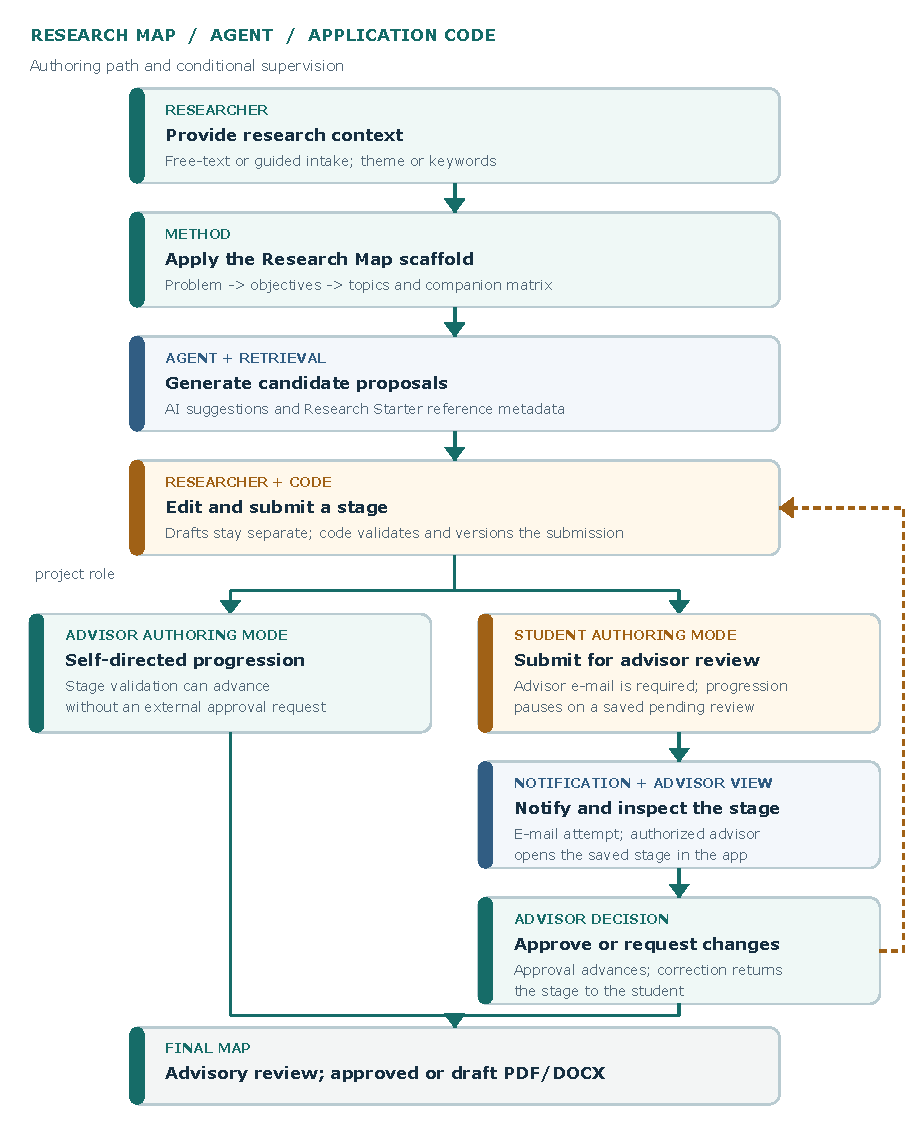
\includegraphics[width=\linewidth]{figures/system-supervision-flowchart.pdf}
\caption{Interpretive flowchart of the Research Map, agent, application code, and conditional student--advisor path in the inspected version-2 workflow. The dashed arrow denotes a request for corrections. E-mail is an attempted notification; the authenticated advisor's in-app decision controls progression. The final algorithmic coherence review remains advisory. This is not an observed user trajectory or a guarantee of scientific quality.}
\label{fig:system-flowchart}
\end{figure}

\subsection{Checks, decisions, and revision}

Validation occurs at different levels. Stage routes check required fields, allowed counts, identifiers, declared topic coverage, and selected lexical relationships. For example, alignment between a problem and an objective can be approximated from wording, while matrix completeness can be checked from filled fields. Neither check establishes that the objective answers the research problem or that a proposed collection and analysis method is appropriate. A product rule also asks for a final development topic linked to the general objective or a stated methodological exception; the latter qualification matters because the source document presents the relation as guidance, not a universal constraint \cite{franca2026detail}.

Drafts and AI proposals are stored separately from the currently confirmed unit, with the source revision from which they were produced. Saving a draft or generating a proposal does not itself replace approved academic content. A confirmation action can update the canonical unit; stale proposals based on an older context require review. Saves use revision matching to avoid silently overwriting a newer version, and changed units have recoverable history.

When confirmed academic content changes, the workflow compares content fingerprints and marks later \emph{types} of elements stale. Earlier text and historical approval remain available for inspection. A change to a literature or development topic can also mark methodology rows stale. This propagation is intentionally conservative: it follows a predefined type-dependency map, not the exact descendants of each stored trace link. The user must revisit affected content and decide what to retain, revise, or confirm.

\subsection{Student and advisor roles}

The application distinguishes the project's \emph{authoring role} from the person who reviews a student's submission. A project authored in advisor mode follows a self-directed path: after applicable stage checks, its author can advance without an external approval request. In student mode, the project must have an advisor e-mail address before a stage can be submitted for advancement, although a draft may still be saved. Submission creates a pending review record for that stage, with its source revision and proposed next state. The stage remains awaiting review and academic confirmation or forward progression is restricted while that request is pending. This applies to submitted units such as the problem, objectives, topic groups, methodology matrix, and final map; it does not mean that every keystroke or initial prompt is individually approved.

After a pending review is saved, the server attempts to notify the registered advisor by e-mail. The message identifies the project and stage and links back to the application. The notification requires a configured mail provider and a usable recipient address; a skipped or failed send does not itself cancel the saved review request. Thus the implementation supports e-mail notification but cannot, from the request path alone, establish delivery to the advisor's inbox or that the message was read. The advisor's review authority comes from authenticated project access in the application, not from possession of the e-mail link.

In the advisor workspace, the reviewer can inspect the submitted stage in the context of the student's map and save a comment, approve it, or request changes. A request for changes requires a comment and returns the stage for student revision and resubmission. Approval records the advisor's decision and applies the pending transition, allowing the student to continue; for the final map, this can establish the current final approval used by the export path. The application also attempts to notify the student of the advisor's comment or decision. This human approval is a product workflow decision and is distinct from the final algorithmic coherence findings described below. Neither author of this paper is represented as having reviewed a student submission for the present descriptive article.

\subsection{Final review and export}

The final map assembles nodes for the input, selected problem, objectives, topics, matrix rows, title, and associated references. Stored trace links and reference associations provide graph edges; deterministic checks can detect orphan edges, cycles, absent elements, and other structural findings. A model-assisted coherence pass adds suggestions or a warning if that pass is unavailable. These findings support inspection. They are not a proof of semantic coherence, feasibility, or likely research outcomes.

The distinction between a check and a completion gate is material. The current completion route invokes the final-map predicate in \emph{advisory} mode, which permits completion despite findings that strict mode would classify as blocking. It then excludes blocking findings from the persisted final summary while retaining non-blocking revision guidance. Earlier stage validation can still reject malformed or incomplete inputs. Accordingly, the present implementation should be described as offering a final traceability and coherence review, not enforcing a guarantee that the completed plan is internally consistent.

For the version-2 workflow, export requires a completed or reviewing map and either current final approval or an explicitly requested draft. PDF and DOCX are rendered from a shared report model without another AI generation call. They contain the proposed research plan, its planned methods and expected results, associated references, and available review warnings. The exported document is a planning artifact; its expected results are not findings from a study. The next section uses a constructed case to make the authoring and revision path concrete without presenting it as user-study evidence.

\section{Constructed illustrative walkthrough}
\label{sec:walkthrough}

The following example is an author-constructed illustration of the relationship between the Research Map and the inspected implementation. It concerns a fictional municipal library and a hypothetical collection of digitized historical photographs. No project was created in the application for this example; no model or Research Starter call was made, no participant supplied data, and no map was completed or exported. The formulations below are illustrative inputs, not responses produced by the agent. This distinction matters because the example can explain a possible authoring path but cannot demonstrate usability, effectiveness, or the quality of a completed research design.

\subsection{Initial synthetic plan}

Suppose that the researcher begins with the question: ``How can metadata standardization support the discovery of historical photographs in a fictional municipal library?'' A corresponding general objective is to analyze how metadata standardization could support discovery in that collection. Three specific objectives are constructed: (OE1) identify descriptive metadata fields; (OE2) examine search patterns in a fictional catalogue; and (OE3) propose guidance for describing and finding the photographs. Three objectives lie within the original map's suggested range of three to six \cite{franca2026map}; their selection here is illustrative, not an agent decision or an author appraisal of methodological adequacy.

The literature outline could contain metadata quality, subject access, and catalogue search. A development outline could contain description of the fictional collection, analysis of constructed search examples, and synthesis of guidance. These are labels for planning relations, not chapters written or sources retrieved. The inspected application represents links between topics and objectives and requires reference identifiers and justifications in its chapter workflow; because this example supplies no real bibliographic records, it is not presented as a set of entries that would pass those routes unchanged.

Table~\ref{tab:walkthrough-matrix} sketches the companion matrix. Every item is prospective. ``Expected output'' refers to an anticipated product of the proposed work, never to an observed result of a library study.

\begin{table}[htbp]
\centering
\small
\caption{Constructed objective--method matrix for the fictional library case. No records, searches, or outputs were collected or produced.}
\label{tab:walkthrough-matrix}
\begin{tabular}{>{\raggedright\arraybackslash}p{0.22\linewidth} >{\raggedright\arraybackslash}p{0.34\linewidth} >{\raggedright\arraybackslash}p{0.34\linewidth}}
\hline
Objective & Planned information and treatment & Expected output \\
\hline
OE1: metadata fields & Constructed catalogue records; compare field presence and consistency & Inventory of fields and candidate gaps \\
OE2: search patterns & Constructed catalogue queries; classify query paths and retrieval descriptions & Map of possible discovery paths \\
OE3: guidance & Planned synthesis of OE1/OE2 and literature still to be verified & Draft rules for description and discovery \\
\hline
\end{tabular}
\end{table}

The actual application additionally stores a methodological classification and a general-objective synthesis row. They are omitted from this compact example, which is intended to explain the relation between specific aims and prospective means, rather than simulate a valid route submission. Whether the proposed inputs or treatments are appropriate would require a disciplinary judgment by a researcher.

\subsection{One upstream change}

Now suppose that the researcher narrows the question to: ``How can standardizing subject and date metadata support the discovery of historical photographs in a fictional municipal library?'' The revision specifies two metadata dimensions that the original question left open. It is not, by itself, evidence that the new question is better. It creates a reason to reconsider whether the general objective, each specific objective, the literature and development topics, and the matrix still address the selected problem.

The implementation distinguishes saving this wording as a draft from confirming it as academic content. Only a confirmed change to the problem triggers the versioned workflow's dependency handling. Its type-level rule can mark the general objective, specific objectives, topics, methodology, title, and final map as stale while retaining their text and history. It does not traverse each trace link to determine which particular sentence is affected. The researcher must inspect those items and decide whether to edit or reaffirm them. Figure~\ref{fig:walkthrough-revision} displays this hypothetical revision and its code-inspected consequence; no such action was executed on the fictional project.

\begin{figure}[htbp]
\centering
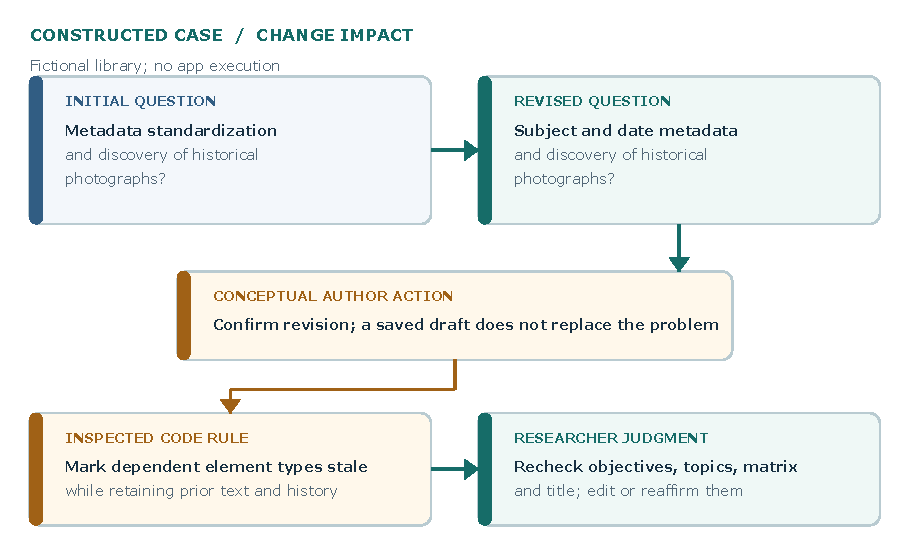
\includegraphics[width=\linewidth]{figures/walkthrough-revision.pdf}
\caption{Constructed change-impact illustration. The initial and revised questions are author-written examples. The stale-marking rule is based on inspected source code, but it was not run on this fictional project. The arrows do not represent observed user behavior or a generated response.}
\label{fig:walkthrough-revision}
\end{figure}

If the same example were entered in student authoring mode, submitting a validated stage would create a pending advisor review and an attempted e-mail notification, as described in Section~\ref{sec:system}. An authenticated advisor could approve the stage or request corrections; approval, rather than the e-mail, would permit the next transition. This conditional branch is included to explain the available workflow. No student submission, message delivery, advisor decision, or methodological rating occurred in this example. In advisor authoring mode, the external review request would not be required.

\subsection{What the illustration demonstrates}

The example makes two relations visible: the map decomposes a central question into objectives, topic structures, and prospective methods; and an upstream edit in the application calls for renewed human consideration of downstream content. The first relation comes from the method's planning documents \cite{franca2026map,franca2026detail}; the second is a behavior supported by inspection of the versioned workflow code, not by execution of this constructed case. The limited local wording checks previously performed on the example found no structural or lexical messages for the revised problem and objectives. They did not validate the topics, matrix, persistence route, coherence of the research design, or any participant outcome.

Final-map review would be advisory, and a PDF or DOCX would require an eligible workflow state and either current final approval or an explicitly labelled draft. No such report was generated for this example. Thus the walkthrough explains a traceable design and a possible revision path; it does not establish that the agent improves planning, that an e-mail was received, or that the hypothetical library project would yield its expected outputs.

\section{Discussion and limitations}
\label{sec:discussion}

\subsection{Contribution in relation to existing work}

The contribution described here is a specific correspondence between a planning method and its software representation. The Research Map relates a problem, objectives, literature and development topics, and an objective--method matrix; the inspected application makes these units editable, records proposals and confirmations separately, and calls attention to later units when an earlier one changes. Its agent assists in formulating and revising content within that structure. The constructed walkthrough shows how the correspondence can be read, rather than how successfully people use it. This is a design and implementation account, not a claim that the Research Map originated staged planning, human review, provenance, or AI-supported research ideation.

The closest methodological papers establish why those broad features cannot serve as novelty claims. Research LLM describes a human-in-the-loop research companion across broader phases \cite{guerard2026researchllm}; Wang et al. organize AI assistance for clinical question formulation in five stages \cite{wang2026fivestage}. The present article instead specifies the Research Map's own units and their interdependencies, including the companion matrix, and examines their translation into application states and checks. CoQuest concentrates on co-creating research questions and reports a researcher study \cite{liu2024coquest}; ResearchAgent and the biomedical system of Aamer et al. explore agentic idea development, critique, knowledge structures, or memory \cite{baek2025researchagent,aamer2026biomedical}. Their empirical findings cannot be transferred to this implementation. Conversely, the present system has no dedicated research-questions unit, so its coverage of that task is narrower than a label such as ``research-question agent'' would suggest.

Workflow-history and provenance work provides another necessary boundary. VisTrails and RaivenTracks make revisions or branches of computational work inspectable, while PROV-DM supplies a general model for describing provenance \cite{freire2006vistrails,hugie2026raiventracks,moreau2013prov}. The Research Map application retains revisions and explicit planning links, but its stale marking follows predefined element types. It neither computes exact impact along each stored link nor demonstrates compliance with PROV-DM. Public descriptions of planning products, particularly ProjectReady AI and Researchly AI, also report overlapping planning or revision assistance \cite{projectready2026guide,researchly2026site}. As those descriptions were not tested in authenticated workflows for this article, the comparison supports a narrow positioning of the documented method--system mapping, not a claim of product priority or feature exclusivity.

The application also exposes a useful distinction within ``human supervision.'' The researcher can inspect and confirm proposed academic content; in student authoring mode, a submitted stage enters a pending review that an authenticated advisor can approve or return with comments. The agent's suggestion, the author's confirmation, the advisor's workflow decision, and scientific validation are different acts. An attempted e-mail notification helps bring a pending review to the advisor's attention, but delivery or reading is not established by the inspected route. This distinction matters when interpreting the flowchart in Section~\ref{sec:system}: its arrows specify possible transitions and responsibilities, not observed use or proof of research quality.

\subsection{Limits of the implementation and evidence}

Several method-to-system correspondences remain partial. The detailed method specification includes research questions among items to validate, whereas the inspected schema places question wording in problem candidates without a separate research-questions unit \cite{franca2026detail}. Topic coverage and trace links record declared relationships; lexical alignment and field-completeness checks cannot decide whether a question is worthwhile, a source supports a claim, or a method can answer an objective. The present suggestion library is static rather than a demonstrated growing methodological knowledge base. Bibliographic identifiers and provider metadata aid identification, but do not verify the relevance or evidentiary support of a cited work.

Revision handling is similarly bounded. Confirming changed content can mark downstream element \emph{types} stale and preserve prior versions, thereby prompting reconsideration. This conservative rule may call for review of unaffected items and cannot prove that every substantively affected relation has been found. At finalization, the route uses an advisory completion predicate and omits blocking findings from its persisted summary. A completed or exported map must therefore not be read as a certificate of coherence. Earlier stage checks and student--advisor approval can constrain transitions, but neither substitutes for disciplinary judgment about the research plan.

The evidence in this article consists of the source method documents, a directed comparison with published work and public product descriptions, inspection of the relevant implementation and local technical checks, and one constructed illustration. The checks support selected statements about program behavior at the examined layers; they are not a complete end-to-end test of every database, notification, agent, and export path. The fictional library case was not entered into the application and contains no generated agent output or observed advisor review. There are no participants, measured completion times, methodological ratings by the authors, or comparisons with an alternative planning process. Consequently, this article cannot establish that the system improves research quality, reduces delays, saves time, or is usable in routine supervision. Its claims concern documented design and inspected capabilities at the examined revision.

\subsection{Implications for further work}

The immediate design implication is to keep proposal, confirmation, review, and evidence status visible as separate information. More precise dependency tracking, explicit handling of unresolved final findings, verification of bibliographic support, and observable notification delivery would make the implementation's claims easier to inspect. These are possible extensions, not features demonstrated here. A separate empirical study could examine how researchers and advisors understand the map and its warnings, and whether the workflow changes planning decisions or effort. Such a study would require its own protocol and data; it is outside the evidentiary scope of this method-and-system article.

\section{Conclusion}
\label{sec:conclusion}

This article has described the Research Map as a method for structuring a research plan and examined how its planning relations are represented in an AI-assisted application. The method connects a central problem to objectives, literature and development topics, and a companion objective--method matrix. In the inspected implementation, the agent proposes content within this structure, while the researcher can edit and confirm it. Versioned records, declared links, stage checks, and review states make parts of that process inspectable. Student-authored submissions can additionally pass through an advisor's in-app decision before progression. These correspondences specify what the system supports; they do not establish the scientific adequacy of a plan.

The fictional library example illustrated one possible revision of a research problem and the need to reconsider dependent planning units. It was deliberately constructed rather than run as an application session. Together with the directed literature comparison and source-code inspection, it supports a bounded contribution: a documented account of how this particular planning method is operationalized in a supervised authoring workflow. Related research systems and public applications already offer staged assistance, agentic ideation, revision history, or planning support. The contribution therefore lies in the documented correspondence and its limits, rather than in a claim of exclusive features or demonstrated improvement over those systems.

The present evidence cannot show that the Research Map improves research quality, reduces effort, or works well in routine supervision. Its automated checks are partial, final coherence review is advisory, bibliographic metadata do not verify support for claims, and the constructed case contains no user or advisor observations. The resulting map and its exports should be interpreted as revisable planning artifacts that remain subject to researcher and advisor judgment. Empirical assessment of use and outcomes would require a separate study.


\section*{Declarations}
\addcontentsline{toc}{section}{Declarations}
\outlinenote{Author contributions, use of AI, data/code availability, funding, conflicts of interest, and supplementary material; complete only after coauthor and journal review.}

{\small
\addcontentsline{toc}{section}{References}
\bibliographystyle{plain}
\bibliography{references}
}

\end{document}
